\documentclass[tikz,border=12pt]{standalone}
\usepackage[T1]{fontenc}
\usepackage{mathpazo}
\usepackage{amsmath,amssymb}
\usetikzlibrary{arrows.meta, positioning, calc, decorations.pathreplacing}

\definecolor{stblue}{HTML}{7B97AD}
\definecolor{rwgold}{HTML}{B8995E}
\definecolor{sage}{HTML}{7A9A7E}
\definecolor{dkbrown}{HTML}{3D3530}
\definecolor{wmgray}{HTML}{7B7067}
\definecolor{cream}{HTML}{F9F6F0}
\definecolor{border}{HTML}{D4C9B8}
\definecolor{terracotta}{HTML}{C47A6A}
\definecolor{lavender}{HTML}{907EA0}

\begin{document}
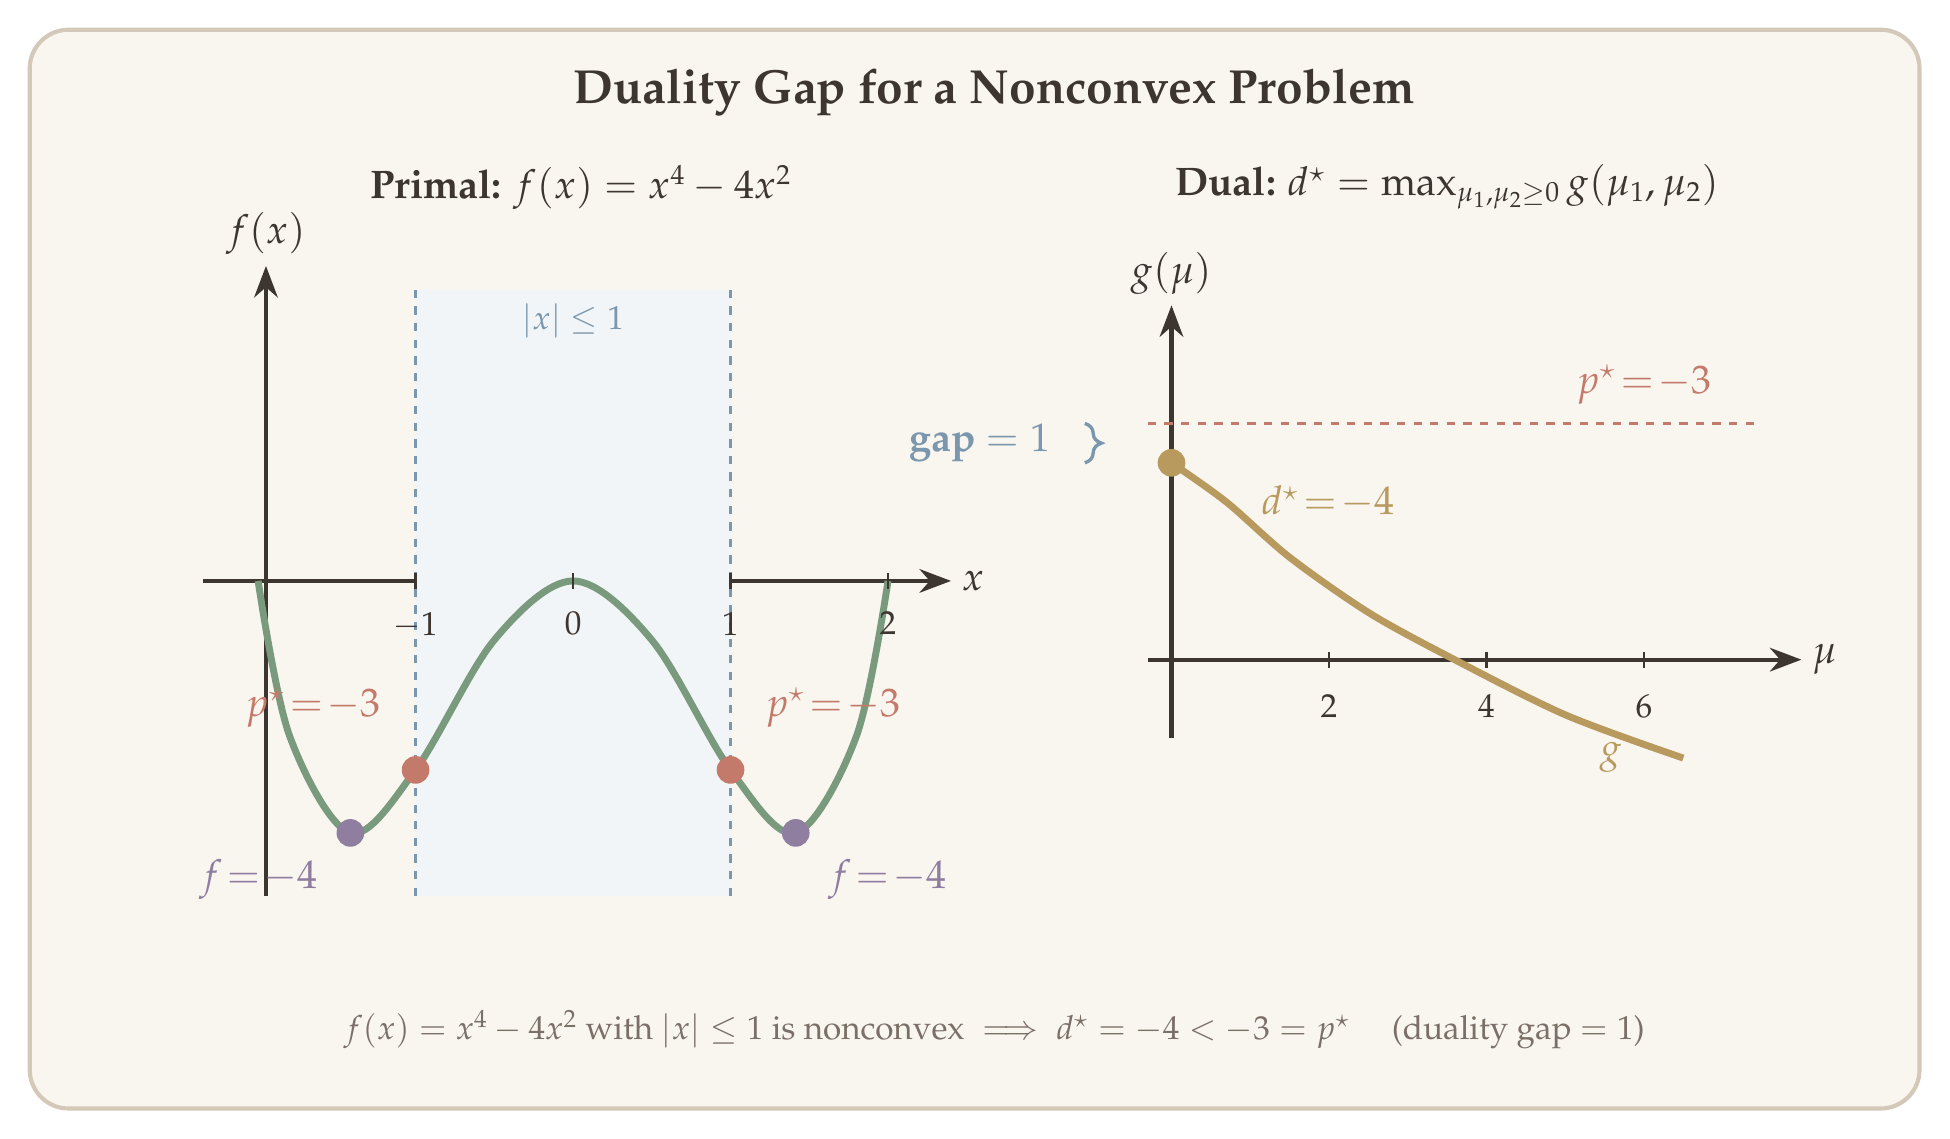
\begin{tikzpicture}[>={Stealth[length=4mm, width=3mm]}, line width=1.5pt]

% Background
\fill[cream, rounded corners=14pt] (-2.5,-4.2) rectangle (21.5,9.5);
\draw[border, line width=1.5pt, rounded corners=14pt] (-2.5,-4.2) rectangle (21.5,9.5);

% Title
\node[font=\LARGE\bfseries, text=dkbrown, align=center] at (9.75,8.7)
  {Duality Gap for a Nonconvex Problem};

% ================================================================
% LEFT PANEL: Primal  f(x) = x^4 - 4x^2,  constraint |x| <= 1
% ================================================================
\begin{scope}[shift={(0,0)}]

% Panel label — positioned above plot area, clear of axis label
\node[font=\Large\bfseries, text=dkbrown] at (4.5,7.5)
  {Primal: $f(x)=x^4-4x^2$};

% Axes — y-axis at tikz x=1, x-axis at tikz y=2.5 (so f=0 lives at y=2.5)
% Coordinate mapping:
%   real x in [-2.2, 2.2] -> tikz X in [0, 8.8]   scale = 2.0 per unit
%     tikz X = (x+2.2)*2.0
%     x=-2.2->0, x=-1->2.4, x=0->4.4, x=1->6.4, x=2->8.4, x=2.2->8.8
%   real f in [-4.5, 5] -> tikz Y: zero at 2.5, scale 0.8 per unit
%     tikz Y = 2.5 + 0.8*f
%     f=0->2.5, f=-3->0.1, f=-4->-0.7, f=4->5.7

\draw[->, dkbrown, line width=1.5pt] (-0.3,2.5) -- (9.2,2.5)
  node[right, font=\Large, text=dkbrown] {$x$};
\draw[->, dkbrown, line width=1.5pt] (0.5,-1.5) -- (0.5,6.5)
  node[above, font=\Large, text=dkbrown] {$f(x)$};

% Feasible region |x| <= 1 shading
% x=-1 -> tikzX = 2.4,  x=1 -> tikzX = 6.4
\fill[stblue!10] (2.4,-1.5) rectangle (6.4,6.2);
\node[font=\large, text=stblue] at (4.4,5.8) {$|x| \le 1$};

% Vertical dashed lines at x = -1 and x = 1
\draw[stblue, dashed, line width=1pt] (2.4,-1.5) -- (2.4,6.2);
\draw[stblue, dashed, line width=1pt] (6.4,-1.5) -- (6.4,6.2);

% Plot f(x) = x^4 - 4x^2
% x=-2.0: f=0      tikzX=0.4, tikzY=2.5
% x=-1.8: f=-2.46  tikzX=0.8, tikzY=0.532
% x=-1.414: f=-4   tikzX=1.572, tikzY=-0.7
% x=-1.0: f=-3     tikzX=2.4, tikzY=0.1
% x=-0.5: f=-0.94  tikzX=3.4, tikzY=1.75
% x=0: f=0         tikzX=4.4, tikzY=2.5
% x=0.5: f=-0.94   tikzX=5.4, tikzY=1.75
% x=1.0: f=-3      tikzX=6.4, tikzY=0.1
% x=1.414: f=-4    tikzX=7.228, tikzY=-0.7
% x=1.8: f=-2.46   tikzX=8.0, tikzY=0.532
% x=2.0: f=0       tikzX=8.4, tikzY=2.5

\draw[sage, line width=2.5pt] plot[smooth, tension=0.55] coordinates {
  (0.4,2.5) (0.8,0.532) (1.572,-0.7) (2.4,0.1)
  (3.4,1.75) (4.4,2.5) (5.4,1.75) (6.4,0.1) (7.228,-0.7)
  (8.0,0.532) (8.4,2.5)
};

% Mark p* = -3 at x = +-1 (both endpoints of feasible region)
\fill[terracotta] (2.4,0.1) circle (5pt);
\node[font=\Large\bfseries, text=terracotta, anchor=south east] at (2.1,0.5)
  {$p^\star\!=\!-3$};
\fill[terracotta] (6.4,0.1) circle (5pt);
\node[font=\Large\bfseries, text=terracotta, anchor=south west] at (6.7,0.5)
  {$p^\star\!=\!-3$};

% Mark unconstrained minima at x = +-sqrt(2) where f=-4
\fill[lavender] (1.572,-0.7) circle (5pt);
\node[font=\Large\bfseries, text=lavender, anchor=north east] at (1.3,-0.9) {$f\!=\!-4$};

\fill[lavender] (7.228,-0.7) circle (5pt);
\node[font=\Large\bfseries, text=lavender, anchor=north west] at (7.5,-0.9) {$f\!=\!-4$};

% x-axis ticks (on the horizontal axis at y=2.5)
\foreach \rx/\tx/\lab in {-1/2.4/{-1}, 0/4.4/{0}, 1/6.4/{1}, 2/8.4/{2}} {
  \draw[dkbrown, line width=0.8pt] (\tx,2.4) -- (\tx,2.6);
  \node[font=\large, text=dkbrown, below] at (\tx,2.25) {$\lab$};
}

\end{scope}

% ================================================================
% RIGHT PANEL: Dual  g(mu1, mu2) = inf_x { x^4 - 4x^2 + mu1(x-1) + mu2(-x-1) }
% ================================================================
\begin{scope}[shift={(11.5,0)}]

% Panel label
\node[font=\Large\bfseries, text=dkbrown, align=center] at (4,7.5)
  {Dual: $d^\star = \max_{\mu_1,\mu_2 \ge 0} g(\mu_1,\mu_2)$};

% Axes — g-axis on left, mu-axis horizontal
% mu in [0,7] -> tikzX [0.5, 8]  scale 1.0
% g values: g(0)=-4 is the max, so map g=-4 -> tikzY=4, scale 0.5/unit downward
%   tikzY = 4 + 0.5*(g+4)
%   g=-4 -> 4, g=-6 -> 3, g=-8 -> 2, g=-10 -> 1, g=-3 -> 4.5

\draw[->, dkbrown, line width=1.5pt] (0.2,1.5) -- (8.5,1.5)
  node[right, font=\Large, text=dkbrown] {$\mu$};
\draw[->, dkbrown, line width=1.5pt] (0.5,0.5) -- (0.5,6)
  node[above, font=\Large, text=dkbrown] {$g(\mu)$};

% p* = -3 -> tikzY = 4 + 0.5*(-3+4) = 4.5
% d* = g(0) = -4 -> tikzY = 4.0

% Plot dual function g(mu): decreasing from mu=0
% g(0)=-4 -> Y=4.0;  g(1)~-6.4 -> Y=2.8;  g(2)~-8.9 -> Y=1.55;
% g(3)~-11.5 -> Y=0.25
\draw[rwgold, line width=2.5pt] plot[smooth, tension=0.5] coordinates {
  (0.5,4.0) (1.2,3.5) (2.0,2.8) (3.0,2.1) (4.0,1.55) (5.5,0.8) (7.0,0.25)
};

% Draw p* line
\draw[terracotta, dashed, line width=1pt] (0.2,4.5) -- (8,4.5);
\node[font=\Large\bfseries, text=terracotta, anchor=south west] at (5.5,4.6) {$p^\star\!=\!-3$};

% Mark d* = g(0) = -4 — dot, with label to the right
\fill[rwgold] (0.5,4.0) circle (5pt);
\node[font=\Large\bfseries, text=rwgold, anchor=west] at (1.5,3.5) {$d^\star\!=\!-4$};

% Brace for duality gap on left side of Y-axis — offset further from y-axis
\draw[decorate, decoration={brace, amplitude=6pt, mirror}, stblue, line width=1.2pt]
  (-0.6,4.0) -- (-0.6,4.5);
\node[font=\Large\bfseries, text=stblue, anchor=east] at (-0.9,4.25) {gap $=1$};

% Tick marks on mu axis
\draw[dkbrown, line width=0.8pt] (2.5,1.4) -- (2.5,1.6);
\node[font=\large, text=dkbrown, below] at (2.5,1.2) {$2$};
\draw[dkbrown, line width=0.8pt] (4.5,1.4) -- (4.5,1.6);
\node[font=\large, text=dkbrown, below] at (4.5,1.2) {$4$};
\draw[dkbrown, line width=0.8pt] (6.5,1.4) -- (6.5,1.6);
\node[font=\large, text=dkbrown, below] at (6.5,1.2) {$6$};

% g label — placed along the curve (schematic cross-section)
\node[font=\Large, text=rwgold, anchor=north west] at (5.8,0.6) {$g$};

\end{scope}

% Bottom annotation
\node[font=\large, text=wmgray, align=center] at (9.75,-3.2)
  {$f(x)=x^4-4x^2$ with $|x|\le 1$ is nonconvex $\implies$ $d^\star = -4 < -3 = p^\star$ \quad (duality gap $= 1$)};

\end{tikzpicture}
\end{document}
